\documentclass{article}
\title{InfluentialInvestmentPrediction: Midterm Report}
\author{Joyce Chen, Lingrui Li, Aleah Kennedy}
\usepackage[utf8]{inputenc}
\usepackage{graphicx}
\usepackage{float}
\begin{document}
\maketitle
\section*{Data Collection Methods}
Our datasets came initially from the SEC (The U.S. Securities and Exchange Commission) Edgar database of 13-F forms. We chose to focus our project specifically on investments made by Goldman Sachs. We downloaded the info tables contained in the 13-F/HA forms as XML documents and converted these to CSV files. The data obtained from the SEC contained data about Golman's holding in companies at the end of each quarter including the type of holding, the authorities through which it was obtained, the amount of the holdings in number of stocks and in monetary amount. 
\section*{Cleaning Data}

We used the pandas python library to convert the CSV files into DataFrames so that we could remove rows and columns we didn't want. Particularly, from looking at the data we decided to ignore data about puts and calls on stocks as they would cause different behavior than other transactions. We also chose to ignore holdings that were not shares (aka the ones with type "PRN"). Then, we combined all duplicate entries under the same issuer by adding them up. We added a column listing the stock price of company that was invested in by dividing the holding monetary value by the number of stocks. The merge we did next gave us columns in a single table for all of the values over each table we got from the SEC. One of the nice aspects of our data is that the values are numeric, only reported data was included in the SEC tables, so we didn't have any missing data. However, we did have to account for the possbility of different companies appearing in the data tables for different quarters. We accomplished this by creating a join on the table that retained only those companies that appeared in every sub table from the quarters we were looking at.
\section*{Final Dataset Features}The final step was to use the holdings amounts over different quarters to calculate changes between consecutive quarters.

Our final dataset columns Company, as well as (4-digit date)amt, (4-digit date)price, and columns for the differences in amts between quarters.Some of the differences are negative, indicating a net sale of stocks by Golman Sachs in that particular company, while positive indicates a net acquisition of stock in that company over the period of the quarter. We can therefore use the stock price from the end of the subsequent quarter to tell if there was a change following the buy/sell.\\

\section*{Initial Data Analysis}

One of the important things left to do with our data was to pick what number of stocks constitutes an "influential" investment. We decided to count the number of times data points from the difference columns appeared in different ranges to get an idea of how much Golman Sachs tended to invest within a quarter. \\
\begin{figure}[H]
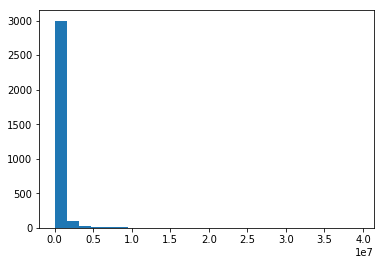
\includegraphics{Unknown.png}
\end{figure}
However, we quickly discovered that some very large investments made it hard to tell where to draw the lower limit. We decided to exclude the extremely high levels and look again.\\
\begin{figure}[H]
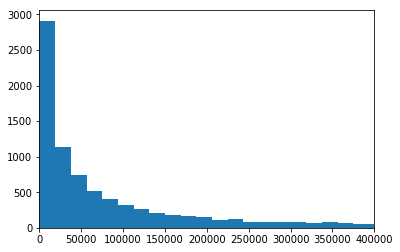
\includegraphics{histogram2.png}
\end{figure}
This plot made choosing a lower cutoff for "influential" difficult as there was no clear break in the data or peak at a non-zero value. We had to use our own discretion instead and we chose to exclude the lower end of the data by setting the lower limit at 200,000 as the absolute value in change of amount of stock held. \\
\begin{figure}[H]
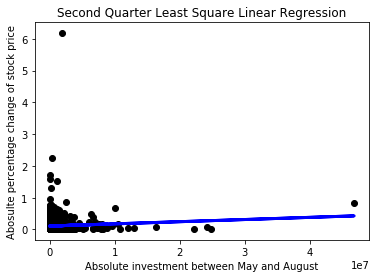
\includegraphics{2.png}
\end{figure}
So far we have run early linear regression models to see if there is a quarterly correlation between the change in amount held over the quarter, and the price of the stock over that same quarter. We found that, with a linear fit, we did get the positive trend we expected but also realized that the less investment was made, the smaller the influence the investment had on the price. 




\section*{Future Work}

In addition to these changes, we would like to try using decision trees on our data with different depths as well. Additionally, we plan to train models on different training sets. Specifically, we can use our cleaning scripts on SEC files from 2015, and 2016 and train on these years, as well as on sets of quarterly data that spans years. After we have different models, we will use cross validation to find the in-sample and out-of-sample errors for these. We will pick the best performing models and create a new model that is the average of these and see how its performance stacks up to the ones it is an aggregate of, based on a test set composed of the data from the first available quarters of 2017.
\end{document}
